
\begingroup
\frametitle{ Neuronale Netze: Black Box?}
\begin{frame}[plain]
	\centering
	
	\begin{tikzpicture}[scale=1, every node/.style={font=\small}]
		% Input Text
		\node at (-5.5, 2) {Input $x \in \mathbb{R}^n$};
		
		% Pfeil von Input zum Hut
		\draw[very thick, ->] (-3,2) -- (-1.8,2);
		
		% Magic Hat Image
		\node at (0, 2.6) {
\includegraphics[width=2.2cm]{BilderPräsentation/magic_hat.png}};
		\node at (0, 1.3) {\footnotesize Neural Network};
		
		% Pfeil von Hut zu Output
		\draw[very thick, ->] (1.4,2) -- (2.8,2);
		
		% Output Text
		\node at (5.2, 2) {Output $g(x)$};
	\end{tikzpicture}
	
	\vspace{1.5em}
	\textbf{Frage:} Können neuronale Netze wirklich jede Funktion lernen?
	
	\vspace{1em}
	{\small\textit{(Spoiler: Ja. Sie sind dicht in $C([0,1]^n)$.)}}
	
\end{frame}
\endgroup

\begingroup
\frametitle{ Universal Approximation Theorem}
\begin{frame}
	\centering
	\begin{tikzpicture}[baseline=(current bounding box.center)]
		% Hutbild
		\node (hat) at (0, 0) {
\includegraphics[width=2.2cm]{BilderPräsentation/magic_hat.png}};
		
		% Beschriftung unter dem Hut
		\node[below=0.5em of hat] {\small \textit{Universal Approximation Theorem}};
		
		% Formelkasten rechts daneben
		\node[anchor=west] (box) at (3.2, 0) {
			\begin{tcolorbox}[colback=blue!5!white,
				colframe=blue!75!black,
				boxrule=0.6pt,
				sharp corners,
				width=0.7\linewidth,
				halign=left]
				\small
				Für jede stetige Funktion $f \in C([0,1]^n)$ und jedes $\varepsilon > 0$
				existiert ein neuronales Netz $g$ der Form:
				\[
				g(x) = \sum_{j=1}^{m} w^{(2)}_j\, \sigma\big( x^\top w^{(1)}_j - b_j \big)
				\]
				sodass $\|f - g\|_\infty < \varepsilon$.
			\end{tcolorbox}
		};
		
		% Quelle unter der Formelbox
		\node[anchor=north west] at (box.south west) {
			\tiny \textit{Quelle:} G. Cybenko, “Approximation by superpositions of a sigmoidal function”, \textit{Mathematics of Control, Signals and Systems}, 1989.
		};	
	\end{tikzpicture}
\end{frame}
\endgroup


\begingroup
\frametitle{Was sind neuronale Netze?}
\begin{frame}[plain]
	\begin{minipage}[t]{0.48\linewidth}
		\vspace*{-0.5em}
		\begin{itemize}
			\item Datengesteuerte, nichtlineare Funktionsapproximation
			\item Aufbau aus Layern und Aktivierungsfunktionen
			\item Lernen durch Backpropagation
		\end{itemize}
	\end{minipage}
	\hfill
	\begin{minipage}[t]{0.50\linewidth}
		\vspace*{-0.5em}
		\centering
		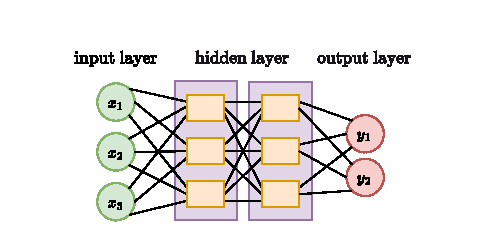
\includegraphics[width=\linewidth]{BilderPräsentation/NN_ausgerichtet.drawio.pdf}
	\end{minipage}
\end{frame}

\endgroup


% Similarity Analysis
\section{Similarity Analysis of Neural Networks}

\begin{frame}
	
	\begin{minipage}[t]{0.49\linewidth}
		\vspace*{-0.5em}
		{\raggedright
			\textbf{\normalsize Ziel der Similarity Analysis} \\[1em]
			\begin{itemize}
				\item Vergleich der internen Repräsentationen zweier Modelle
				\item Zwei Perspektiven:
				\begin{itemize}
					\item Representational Similarity
					\item Functional Similarity
				\end{itemize}
			\end{itemize}
		}
	\end{minipage}
	\hfill
	\begin{minipage}[t]{0.48\linewidth}
		\vspace*{-0.5em}
		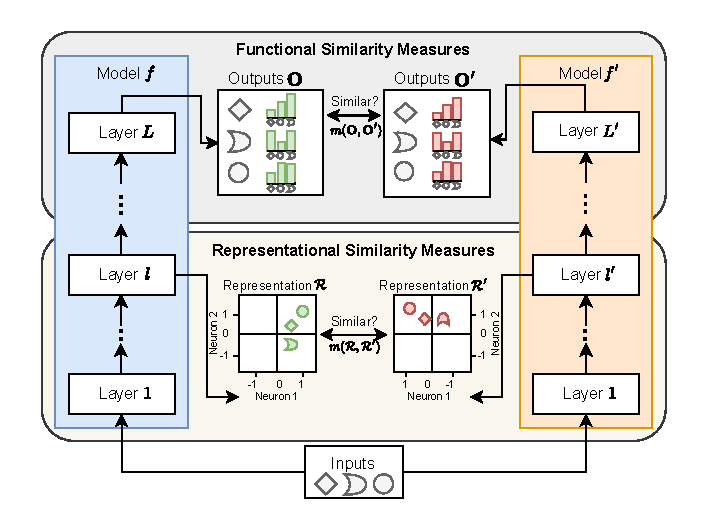
\includegraphics[width=\linewidth]{BilderPräsentation/Similarity90Deg.drawio.pdf}
	\end{minipage}
	
\end{frame}



% Intrinsic Homotopy
\section{Intrinsic Homotopy}
\begin{frame}
	\textbf{Was ist Intrinsic Homotopy?}\\
	\begin{itemize}
		\item Nichtlineare Transformation zwischen Repräsentationen zweier Modelle
		\item Idee: Modell A kann in Modell B deformiert werden
		\item Formalisierung über Hemi-Metriken und Homotopie-Pfade
	\end{itemize}
\end{frame}

% Implementierung
\section{Implementierung}
\begin{frame}
	\textbf{Praktische Umsetzung in PyTorch}\\
	\begin{itemize}
		\item Nichtlineare Netze mit Spectral Normalization
		\item Training auf $\ell^\infty$-Fehler
		\item Analyse von Lipschitz-Konstanten und Spearman-Korrelation
	\end{itemize}
\end{frame}

% Experimente
\section{Experimente}
\begin{frame}
	\textbf{Experimente zur Intrinsischen Homotopie}\\
	\begin{itemize}
		\item Setup: MULTIBERT, ROBERTA, ELECTRA
		\item Evaluation mit Repräsentationen auf GLUE-Tasks
		\item Visualisierung der Pfadlängen und Korellationen
	\end{itemize}
\end{frame}

% Fazit
\section{Fazit und Ausblick}
\begin{frame}
	\textbf{Was haben wir gelernt?}\\
	\begin{itemize}
		\item Intrinsische Homotopie bietet tiefen Einblick in Modellstruktur
		\item Kombinierbar mit funktionaler Analyse und Robustheit
		\item Nächste Schritte: Performance-based Homotopy und extrinsischer Vergleich	\end{itemize}
\end{frame}
